% created for ISDA2011 conference http://www.uco.es/isda2011/
% Time-stamp: "2011-06-16 21:02:55 hei2"
% PAPER ISDA2011-
% name: Helga Ingimundardottir
% e-mail: hei2@.is

\documentclass[conference]{IEEEtran}
\usepackage[english]{babel}  
\usepackage{latexsym}
\usepackage{amsmath,amssymb}
\usepackage[dvips]{graphicx,psfrag}

\newcommand{\norm}[1]{\lVert#1\rVert}
\renewcommand{\vec}[1]{{\mbox{\boldmath$#1$}}}
\newcommand{\mat}[1]{{\mbox{\boldmath$#1$}}}
\newcommand{\reals}{{\mathbb R}}
\newcommand{\strng}[1]{{\mbox{\tt #1}}}
\newcommand{\inner}[2]{\big<\vec{#1}\cdot\vec{#2}\big>}

\def\argmax{\mathop{\rm argmax}}
\def\argmin{\mathop{\rm argmin}}
\newcommand\bs{\char '134}   
\usepackage{color}

\usepackage{tabularx}

\renewcommand{\vec}[1]{{\mathbf #1}}
\hyphenpenalty=800
\hbadness=2500

\title{Sampling Strategies in Ordinal Regression for Surrogate Assisted Evolutionary Optimization}

\author{
  \IEEEauthorblockN{Helga Ingimundardottir}
  \IEEEauthorblockA{School of Engineering and Natural Sciences \\University of Iceland\\
    Email: hei2@hi.is 
  }
\and
  \IEEEauthorblockN{Thomas Philip Runarsson}
  \IEEEauthorblockA{School of Engineering and Natural Sciences \\University of Iceland\\
    Email: tpr@hi.is 
   }
}
%\author{Helga Ingimundardottir \and Thomas Philip Runarsson}
%\institute{{Science Institute, University of Iceland}\\
%\email{hei2@hi.is}, \email{tpr@hi.is}}
\begin{document}
\maketitle

%\thispagestyle{empty}\pagestyle{empty}
\selectlanguage{english}

\begin{abstract}
  In evolutionary optimization surrogate models are commonly used when the evaluation of a fitness function is computationally expensive. Here the fitness of individual points are indirectly estimated by modeling their rank with respect to the current population by use of ordinal regression. 
  The paper focuses on how to validate the goodness of fit for surrogate models during search and introduces a novel validation/updating policy for surrogate models, and is illustrated on classical numerical optimization functions for evolutionary computation. The study shows that for validation accuracy it is sufficient for the approximate ranking and true ranking of the training set to be sufficiently concordant or that only the potential parent points should be ranked consistently. Moreover, the new validation approach reduces the number of fitness evaluation needed, without a loss in performance.
\end{abstract}

\section{Introduction}\label{sec:introduction}

Evolutionary optimization is a stochastic and direct search method
where a population of points are searched in parallel.  Typically only
the full or partial ordering of these parallel search points is
needed.  For this reason an ordinal regression offers sufficiently
detailed surrogates for evolutionary computation
\cite{Ru06:PPSN}.  In this case there is no explicit fitness
function defined, but rather an indirect method of evaluating whether
one point is preferable to another.

The current approach in fitness approximation for evolutionary
computation involves building surrogate fitness models directly using
regression.  For a recent review of the state-of-the-art see
\cite{Ong04,SLK05,Jin05,Lim2007}. The fitness model is based
on a set of evaluated points called the training set. The surrogate
model is used to predict the fitness of candidate search
points. Commonly a fraction of points are selected and evaluated
within each generation (or over some number of generations
\cite{JOS02}), added to the training set, and used for updating the
surrogate.  The goal is to reduce the number of costly true fitness
evaluations while retaining a sufficiently accurate surrogate during
evolution. When using ordinal regression a candidate search point
$\vec{x}_i$ is said to be preferred over $\vec{x}_j$ if $\vec{x}_i$
has a higher fitness than $\vec{x}_j$. The training set for the
surrogate model is therefore composed of pairs of points
$(\vec{x}_i,\vec{x}_j)_k$ and a corresponding label $t_k\in[1 ,-1]$,
taking the value $+1$ (or $-1$) when $\vec{x}_i$ has a higher fitness
than $\vec{x}_j$ (or vice versa).  The direct fitness approximation
approach does not make full use of the flexibility inherent in the
ordering requirement. The technique used here for ordinal regression
is kernel based and is described in section~\ref{sec:OR} and was first
presented in \cite{Ru06:PPSN}. The use of surrogate models and approximate 
ranking has made some headway, e.g. \cite{Loshchilov2010}, however still 
remains relatively unexplored field of study.

The critical issue in generating surrogate models, for evolutionary
search, is the manner in which the training set is constructed. For
example, in optimization it is not critical to model accurately regions
of the search space with low fitness. It is, however, key to model
accurately new search regions deemed potentially lucrative by the
evolutionary search method. Furthermore, since the search itself is
stochastic, perhaps the ranking need not be that accurate. Indeed the
best $\mu$ candidate individuals are commonly selected and the rest
disregarded irrespective of their exact ranking.

In the literature new points are added to the training set from the
new generation of unevaluated search points. This seems sensible since
this is the population of points which need to be ranked. However,
perhaps sampling a representative point, for example the mean of the
unevaluated search points, may also be useful in surrogate ranking.
Typically, the unevaluated points are ranked using the current
surrogate model and then the best of these are evaluated using the true
expensive fitness function and added to the training set. Again, this
seems sensible since we are not interesting in low fitness regions of
the search space. Nevertheless, it remains unclear whether this is
actually the case. Finally, there is the question of knowing when to
stop, when is our surrogate sufficiently accurate? Is it necessary to
add new search points to our training set at every search generation?
What do we mean by sufficiently accurate? This paper describes some
preliminary experiments with the aim of investigating some these issues
further.

In section~\ref{sec:samplingstopping} sampling methods, stopping criteria and model accuracy are discussed. Moreover, a strategy for updating the surrogate during search is presented and its effectiveness illustrated using the CMA-ES \cite{hansen:ostermeier:01} on some numerical optimization functions in section~\ref{sec:Experiment}. The paper concludes with discussion and summary in section~\ref{sec:Discussion}.


\section{Ordinal Regression}\label{sec:OR}
Ordinal regression in evolutionary optimization has been previously presented in \cite{Ru06:PPSN} but is given here for completeness. 
%The training pairs are selected to reflect the fact that a full ranking surrogate model is required for the work presented here {\bf ... however late just presented only the mu best ranking pairs need to be ranked correctly}. It is also possible to select the pair by random sampling as is done in \cite{Herbrich00}.
The ranking problem is specified by a set $S = \{(\vec{x}_i,y_i)\}_{i=1}^\ell \subset X \times Y$ of point/rank pairs, where $Y=\{r_1,\ldots,r_\ell\}$ is the outcome space with ordered ranks $r_1> r_2,> \ldots > r_\ell$.   Now consider the model space $\mathcal{H} = \{h(\cdot) : X \mapsto Y\}$ of mappings from points to ranks. Each such function $h$ induces an ordering $\succ$ on the points by the following rule:
\begin{equation}
\vec{x}_i \succ \vec{x}_j \quad \Leftrightarrow \quad h(\vec{x}_i) > h(\vec{x}_j)
\end{equation}
where the symbol $\succ$ denotes ``is preferred to''.  In ordinal regression the task is to obtain function $h^*$ that can for a given pair $(\vec{x}_i,y_i)$ and $(\vec{x}_j,y_j)$ distinguish between two different outcomes: $y_i > y_j$ and $y_j > y_i$. The task is, therefore, transformed into the problem of predicting the relative ordering of all possible pairs of examples \cite{Herbrich00,joachims02}.  However, it is sufficient to consider only all possible pairs of adjacent ranks, see also \cite{shawe-taylor04:book} for yet an alternative formulation.  The training set, composed of pairs, is then as follows:
$$S' = \big\{(\vec{x}_k^{(1)}, \vec{x}_k^{(2)}),t_k=\text{sign}(y_k^{(1)} - y_k^{(2)})\big\}_{k=1}^{\ell'}$$
where $(y_k^{(1)} = r_i) \wedge (y_k^{(2)} = r_{i+1})$ (and vice versa $(y_k^{(1)} = r_{i+1}) \wedge (y_k^{(2)} = r_{i})$) resulting in $\ell'=2(\ell-1)$ possible adjacently ranked training pairs. The rank difference is denoted by $t_k\in[-1,1]$.

In order to generalize the technique to different point data types and model spaces an implicit kernel-defined feature space with corresponding feature mapping $\phi$ is applied. Consider the feature vector $\phi(\vec{x})=[\phi_1(\vec{x}),\ldots,\phi_m(\vec{x})]^T\in
\reals^m$ where $m$ is the number of features. Then the surrogate considered may be defined by a linear function in the kernel-defined feature space:
\begin{equation}
h(\vec{x}) = \sum_{i=1}^m w_i\phi_i(\vec{x}) = \inner{w}{\phi(\vec{x})}.
\end{equation}

The aim now is to find a function $h$ that encounters as few training errors as possible on $S'$. Applying the method of large margin rank boundaries of ordinal regression described in \cite{Herbrich00}, the optimal $\vec{w}^*$ is determined by solving the following task:
\begin{equation} \min_{\vec{w}}\quad \tfrac{1}{2}\inner{w}{w} + \tfrac{C}{2}\sum_{k=1}^{\ell'}\xi_k^2 \label{eq:margin} \end{equation}
subject to $t_k\inner{w}{(\phi(\vec{x}_k^{(1)})-\phi(\vec{x}_k^{(2)})}\ge 1 - \xi_k$ and $\xi_k \ge 0$, $k = 1,\ldots, \ell'$. The degree of constraint violation is given by the margin slack variable $\xi_k$ and when greater than $1$ the corresponding pair are incorrectly ranked. Note that
\begin{equation} h(\vec{x}_i)-h(\vec{x}_j) = \inner{w}{(\phi(\vec{x}_i)-\phi(\vec{x}_j))} \end{equation}
and that minimizing $\inner{w}{w}$ maximizes the margin between rank boundaries, in our case the distance between adjacently ranked pair $h(\vec{x}^{(1)})$ and $h(\vec{x}^{(2)})$.

%In terms of the training data, the optimal $\vec{w}^*$ can be expressed as:
%\begin{equation} \vec{w}^* = \sum_{k=1}^{\ell'}\alpha^*t_k\big(\phi(\vec{x}_k^{(1)})-\phi(\vec{x}_k^{(2)})\big) \end{equation}
%and the function $h$ may be reconstructed as follows:
%\begin{eqnarray} h(\vec{x}) &=& \big<\vec{w}^*\cdot\phi(\vec{x})\big> \\ & = & \sum_{k=1}^{\ell'}\alpha^*t_k\big(\big<\phi(\vec{x}_k^{(1)})\cdot\phi(\vec{x})\big>-\big<\phi(\vec{x}_k^{(2)})\cdot\phi(\vec{x})\big>\big)\nonumber\\ & = & \sum_{k=1}^{\ell'}\alpha^*t_k\big(\kappa(\vec{x}_k^{(1)},\vec{x})-\kappa(\vec{x}_k^{(2)},\vec{x})\big) \end{eqnarray}
%where $\kappa(\vec{x},\vec{z}) = \inner{\phi(\vec{x})}{\phi(\vec{z})}$ is the chosen kernel and $\vec{\alpha}^*_k$ are the Lagrangian multipliers for the constraints that can be determined by solving the dual quadratic programming problem:
%\begin{eqnarray}  \max_{\vec{\alpha}} \quad \sum_{k=1}^{\ell'}\alpha_k-\tfrac{1}{2}\sum_{i=1}^{\ell'}\sum_{j=1}^{\ell'}\alpha_i\alpha_jt_it_j\big( K(\vec{x}_i^{(1)},\vec{x}_i^{(2)},\vec{x}_j^{(1)},\vec{x}_j^{(2)})+\tfrac{1}{C}\delta_{ij}\big) \end{eqnarray}
%subject to $\sum_{k=1}^{\ell'}\alpha_kt_k=0$ and $0\le \alpha_k$, $k = 1,\ldots,\ell'$, where $K(\vec{x}_i^{(1)},\vec{x}_i^{(2)},\vec{x}_j^{(1)},\vec{x}_j^{(2)}) = \kappa(\vec{x}_i^{(1)},\vec{x}_j^{(1)})-\kappa(\vec{x}_i^{(1)},\vec{x}_j^{(2)})-\kappa(\vec{x}_i^{(2)},\vec{x}_j^{(1)})+\kappa(\vec{x}_i^{(2)},\vec{x}_j^{(2)})$, where $\delta_{ij}$ is the Kronecker $\delta$ defined to be $1$ if $i=j$ and $0$ otherwise \cite{CS02:book}. 
Furthermore, it is important to scale the features $\vec{\phi}$ first as the evolutionary search zooms in on a particular region of the search space. A standard method of doing so is by scaling the training set such that all points are in some range, typically $[-1,1]$. That is, scaled $\tilde{\vec{\phi}}$ is
\begin{equation}\label{eq:scale}
\tilde \phi_i = 2 (\phi_i - \underline{\phi}_i) / (\overline{\phi}_i - \underline{\phi}_i) - 1 ~~~ i = 1,\ldots,m
\end{equation}
where $\underline{\phi}_i$, $\overline{\phi}_i$ are the minimum and maximum $i$-th component of all feature vectors in the training set. 

\section{Sampling Methods and Improvements}\label{sec:samplingstopping}
In surrogate modeling a small sample of training points of known fitness are needed to generate an initial surrogate. There after sampling is needed to be conducted for validating and updating the surrogate. Bearing in mind that there is generally a predefined maximum number of expensive function evaluations that can be made, the sampling of test points used for validating/updating the surrogate needs to be fruitful. 

During evolution different regions of the space are sampled and as a consequence the surrogate ranking model may be insufficiently accurate for new regions of the search space, hence if the surrogate is not updated to reflect the original fitness function it is very probable that the ES converges to a false optimum. It is, therefore, of paramount importance to validate the surrogate during evolution, in the literature this is referred to as model management or evolution control. The accuracy can be validated by generating test points in the new region, namely from the new candidate points generated at every generation of the CMA-ES by reproduction, recombination and mutation. The validation control can either be generation based, i.e. when the surrogate is converging, or individual-based, where  at each generation some of the new candidate points are evaluated with the exact model and others are evaluated with the surrogate, see \cite{Jin05}. The selection of points to be evaluated exactly can be done randomly, however, in \cite{Ru04:PPSN} it is reported that validating the accuracy of the ranking of potential parent points during evolution is most beneficial as they are critical for success. For Kriging surrogate model in particular an ``infill sampling criteria'' is implemented by sampling the points which the surrogate believes to be in the vicinity of global optima, however in some cases points in uncertain areas are also explored, this is referred to as generalized expected improvement \cite{Sasena2002}. A performance indicator to which strategy should be focused on, i.e. following the global optima vs. getting rid of uncertainties, \cite{Ponweiser2008} suggests the distance between approximated optima and its real fitness value, however no obvious correlation between the two ranks could be concluded. Moreover, \cite{Ratle1999} compares 6 various sampling procedures for updating the training set using the Kriging model. Two main strategies are explored, mainly evaluating the entire candidate population or only a subset. Latter yielding a significantly fewer exact function evaluations and obtain similar goodness of fit. The former strategy mostly focuses on whether all, partial or none of the training set should be replaced, and whether the outgoing training points should be the worst ranking ones (elitist) or chosen at random (universal), where the elitist perspective was considered more favorable. However, reevaluating a subset of the best ranked points w.r.t. the surrogate model with the exact fitness function yielded the greatest performance edge of the strategies explored. 

When the training accuracy is 100\% one way of evaluating the accuracy of the surrogate is through cross validation. The quality of the surrogate is measured as the rank correlation between the surrogate ranking and the true ranking on training data. Here Kendall's $\tau$ is used for this purpose \cite{kendalltau}.  Kendall's $\tau$ is computed using the relative ordering of the ranks of all $\ell(\ell-1)/2$ possible pairs.  A pair is said to be concordant if the relative ranks of $h(\vec{x}_i)$ and $h(\vec{x}_j)$ is the same for $f(\vec{x}_i)$ and $f(\vec{x}_j)$, otherwise they are discordant. Kendall's $\tau$ is the normalized difference in the number of concordant and discordant pairs, defined as follows,
\begin{equation}
\tau = \frac{C-D}{\sqrt{C+D+T(h)}\sqrt{C+D+T(f)}}
\end{equation}
where $C$ and $D$ denote the number of concordant and discordant pairs, respectively, and $T$ denotes number of ties.
Two rankings are the same when $\tau=1$, completely reversed if $\tau = -1$, and uncorrelated for $\tau \approx 0$.

\begin{figure}[b!]
\centering
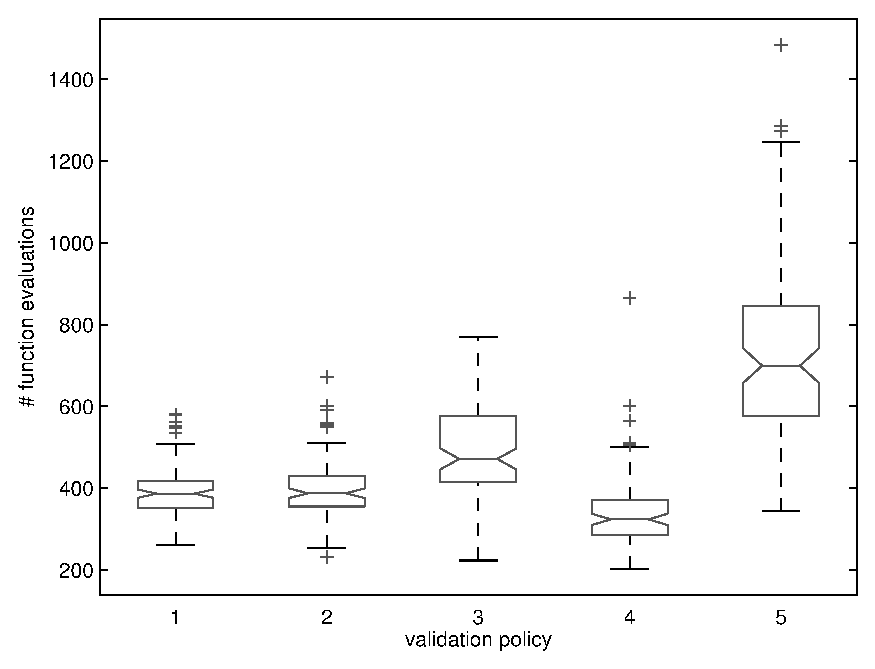
\includegraphics[width=0.95\columnwidth]{figs/anova.eps}
\caption{Anova plot for different validation strategies: 1) prune old points, 2) prune bad points, 3) adding a pseudo mean candidate point 
4) correctly rank $\mu$ best ranked candidate points 5) update on every other generation for the Rosenbrock's function for dimension $n=2$}
\label{fig:anova}
\end{figure}

The surrogate ranking validation and improvement strategy using ordinal regression is tested using the CMA-ES \cite{hansen:ostermeier:01}. The CMA-ES is a very efficient numerical optimization technique but we still expect to reduce the number of function evaluations needed for search. In \cite{Ru06:PPSN} the validation policy had to successfully rank all of the candidate points, i.e. until $\tau=1$, and pruned the training size to $\overline{\ell} = \lambda$ by omitting the oldest points first. These are quite stringent restrictions which can be improved upon. 
% Pruning away the baddest - instead of the oldest 
The pruning only considers the age of the points, however older points might still be of more interest than newer ones if their fitness ranks higher. Thus a more sophisticated way of pruning would be omitting the lowest ranking points first. 
% Validating on a mean pseudo point 
Moreover, the candidate points are generated randomly using a normal distribution, thus a pseudo point representing their mean could be of interest as an indicator for the entire population, e.g. by validating this pseudo point first could give information if the surrogate is outdated w.r.t. the current search space. 
% Validation only the current mu best ranked points
Furthermore, the validation is only done on the candidate points for the current generation in the CMA-ES algorithm where only the $\mu$ best ranked points will survive to become parents. In evolutionary computing one is interested in the accurate ranking of points generated in the neighborhood of parent points, hence for sufficient validation of the surrogate, only the $\mu$ best ranked points should be considered and evaluated, since all other points of lower rank will be disregarded in the next iteration of the CMA-ES. 
% Validating on every other generation
Lastly, one should also investigate the frequency by which the model is validated, e.g. at each generation or every $K>1$ generations or even have the need for validating adapt with time.

Preliminary tests were conducted on which validation method deemed fruitful, by implementing the Rosenbrock's function of dimension $n=2$, for 1) the setup presented in \cite{Ru06:PPSN} and comparing it with the aforementioned validation improvements which were added one at a time, namely: 2) omitting the worst points during the pruning process, instead of the oldest ones; 3) initialize the validation process by using a pseudo point that represents the mean of the new candidate points; 4) requiring that only the $\mu$ best candidate points are correctly ranked; and 5) validating on every other generation. 
Experimental results focusing on the number of function evaluations are shown in Fig.~\ref{fig:anova}. There is no statistical difference between omitting first old or badly ranked points from the training set, but this was expected, since both are believed to be representatives of a region of the search space which is no longer of interest. Adding the pseudo mean candidate point didn't increase the performance edge. When the surrogate was updated on every other generation, it quickly became outdated and more than double function evaluations were needed to achieve the same rate of convergence. 
However requiring the correct ranking for only the $\mu$ best ranked candidate points showed a significant performance edge. 

If the training accuracy is not 100\% then clearly $\tau_t < 1$. In this case additional training points would be forced for evaluation. However, enforcing a completely concordant ranking, i.e. $\tau=1$, was deemed to be too strict due to the fact the search is stochastic. Thus the surrogate is said to be sufficiently accurate if $\tau>0.999$. % Færa kannski frekar upp hjá línu 162, þ.e. áður en mism. valdiation aðferðir eru kynntar?

Based on these preliminary tests, a pseudo code for the proposed model validation and improvement strategy is described in Fig.~\ref{fig:improvedmodel} where it is implemented at the end of each generation of the CMA-ES. The algorithm essentially only evaluates the expensive true fitness function when the surrogate is believed to have diverged. During each iteration of the validation process there are two sets of points, $\mathcal{Y}$ and $\mathcal{X}$, which are the training points which have been evaluated with the expensive model, and the candidate points (of unknown fitness) for the next iteration of the CMA-ES, respectively. The test points of interest are those who are believed to become parent points in the next generation of the CMA-ES algorithm, i.e. the $\mu$ best ranked candidate points according to the surrogate $h$. The method uses only a simple cross-validation on a single test point, the one which the surrogate ranks the highest and has not yet been added to the training set. Creating more test points would be too costly, but plausible. Once a test point has been evaluated it is added to the training set and the surrogate $h$ is updated w.r.t. $\mathcal{Y}$, cf. Fig.~\ref{fig:schema}. If the Kendall's $\tau$ statistic between the ranking of the training set using the surrogate, $\bar{R}$, and its true ranking, $R$, is higher than $0.999$ or if the $\mu$ best ranked candidate points w.r.t. the current surrogate have been added to the training set then the surrogate is said to be sufficiently accurate. Note that during each update of the surrogate the ranking of the $\mu$ best candidate points can change, thus it is possible to evaluate more then $\mu$ test points during each validation. Once the validation algorithm has completed, the training set is pruned to a size $\bar{\ell}=\lambda$ by omitting the lowest ranking points. 

\begin{figure}[t!]
\centering \noindent 
{\footnotesize
\begin{tabbing}
\quad \quad \= 0\;\; \= \emph{Initialization}: Let $\mathcal{Y}$ denote current training set and its \\
\>   \> corresponding surrogate by $h$. Let $\mathcal{X}$ denote population \\
\>   \> of $\lambda$ points of unknown fitness under inspection.\\
\>1  \> {\bf for} \= $t := 1$ to $\lambda$ {\bf do} \emph{(validate test points)}\\ 
\>2  \>\> Estimate ranking of $\mathcal{X}$ using $h$; denoted by $\bar{R}_0$. \\
\>3  \>\> $\vec{x}_B \leftarrow \max_{\vec{x}\in\mathcal{X}\setminus\mathcal{Y}}\left\{\bar{R}_0\right\}$ (\emph{test point}). \\
\>4  \>\> Rank $\vec{x}_B$ w.r.t. points in $\mathcal{Y}$ using $h$; denoted by $\bar{R}$. \\
\>5  \>\> Evaluate $\vec{x}_B$ using true fitness function and evaluate its\\
\>   \>\> true rank among  points in $\mathcal{Y}$; denoted by $R$. \\ 
% In the case where no explicit fitness function can be defined, the test point is evaluated by comparing it with selected points in the training set.
\>6  \>\> $\mathcal{Y}\leftarrow\mathcal{Y}\cup\{\vec{x}_B\}$ \emph{(add to training set)}. \\
\>7  \>\> Compare the rankings  $\bar{R}$ and $R$ by computing the rank \\
\>   \>\> correlation $\tau$.\\
\>8  \>\> {\bf if} \= $\tau>0.999$ {\bf then} \\
\>9  \>\> \> break (\emph{model is sufficiently accurate}) \\
\>10 \>\> {\bf fi} \\
%This is a simple cross-validation on a single test point. Creating more test points would be too costly, but plausible.
\>11  \>\> Update the surrogate $h$ using the new training set $\mathcal{Y}$.\\
\>12  \>\> {\bf if} \= $\mu$ best points of $\bar{R}_0$ have been evaluated {\bf then} \\
\>13  \>\> \> break (\emph{model is sufficiently accurate}). \\
\>14  \>\> {\bf fi} \\
\>15  \> {\bf od}\\
%  Repeated the steps 1-9 above until $\tau_t>0.999$ or at least the $\mu$  highest ranking points of unknown fitness have been evaluated. There is no need to evaluate more than the $\mu$ best ranking points since they will be disregarded in the next iteration of the CMA-ES.
\end{tabbing}}
\caption{Sampling strategy to validate and improve surrogate models.}\label{fig:improvedmodel}
\end{figure}

\begin{figure}[t!]
\centering 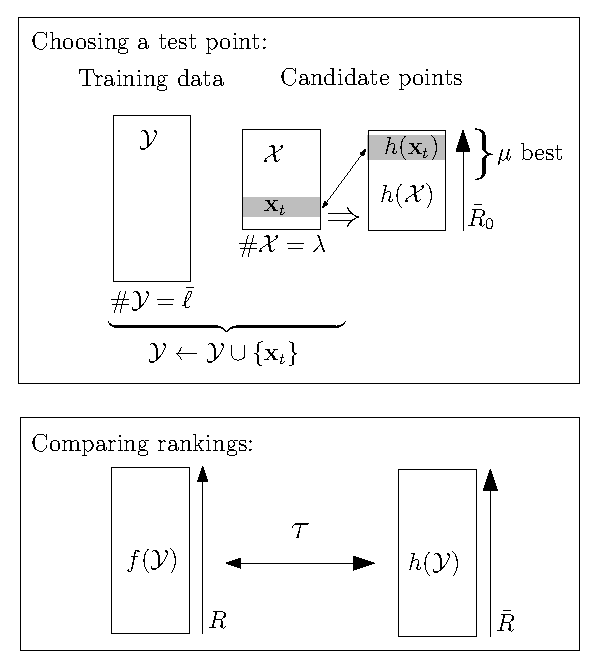
\includegraphics[width=0.7\columnwidth]{figs/schema.eps}
\caption{Schema for the sampling strategy.}\label{fig:schema} 
\end{figure}

\section{Experimental Study}\label{sec:Experiment}
In the experimental study the CMA-ES is run for several test functions, namely the sphere model and Rosenbrock's function, of various dimensions $n=2,5,10$ and $20$. The average fitness for $100$ independent runs versus the number of function evaluations is reported using the original validation procedure presented in \cite{Ru06:PPSN} and compared with its new and improved validation procedure presented in Fig.~\ref{fig:improvedmodel}. %, the procedures will be referred to as using ``all'' or only the ``$\mu$ best'' candidate points during the validation, respectively.
The parameter setting for the $(\mu,\lambda)$ CMA-ES is as recommended in \cite{hansen:ostermeier:01} with population size $\lambda = 4+\lfloor 3\ln(n)\rfloor$ and the number of parents selected $\mu=\lambda/4$. The stopping criteria used are $1000n$ function evaluation or a fitness less than $10^{-10}$. The initial mean search point is generated from a uniform distribution between $0$ and $1$. It is also noted that the training set is only pruned to size $\overline{\ell} = \lambda$ subsequent to the validation and improvement procedure introduced in Fig.~\ref{fig:improvedmodel}. 

\subsection{Sphere model}\label{sec:sphere}
The first experimental results are presented for the unimodal sphere model, 
\begin{equation} f(\vec{x}) = \sum_{i=1}^nx_i^2.\end{equation}
The average fitness versus the number of function evaluations is presented in Fig.~\ref{fig:sphereFitness}. A performance edge is achieved by restricting the validation strategy to only having the surrogate correctly rank the $\mu$ highest ranking points, and thereby saving the algorithm of evaluating points that would have been disregarded in the next iteration. Fig.~\ref{fig:sphereIntmEval} shows the mean intermediate function evaluations that are calculated during the validation process. As one expects requiring the method to evaluate no more than the $\mu$ best ranked candidate points results in a lower intermediate function evaluations, generally saving the method one function evaluation per generation, it also achieves a better mean fitness, as shown in Table~\ref{tbl:Sphere}.

\begin{figure}[b!]
\centering
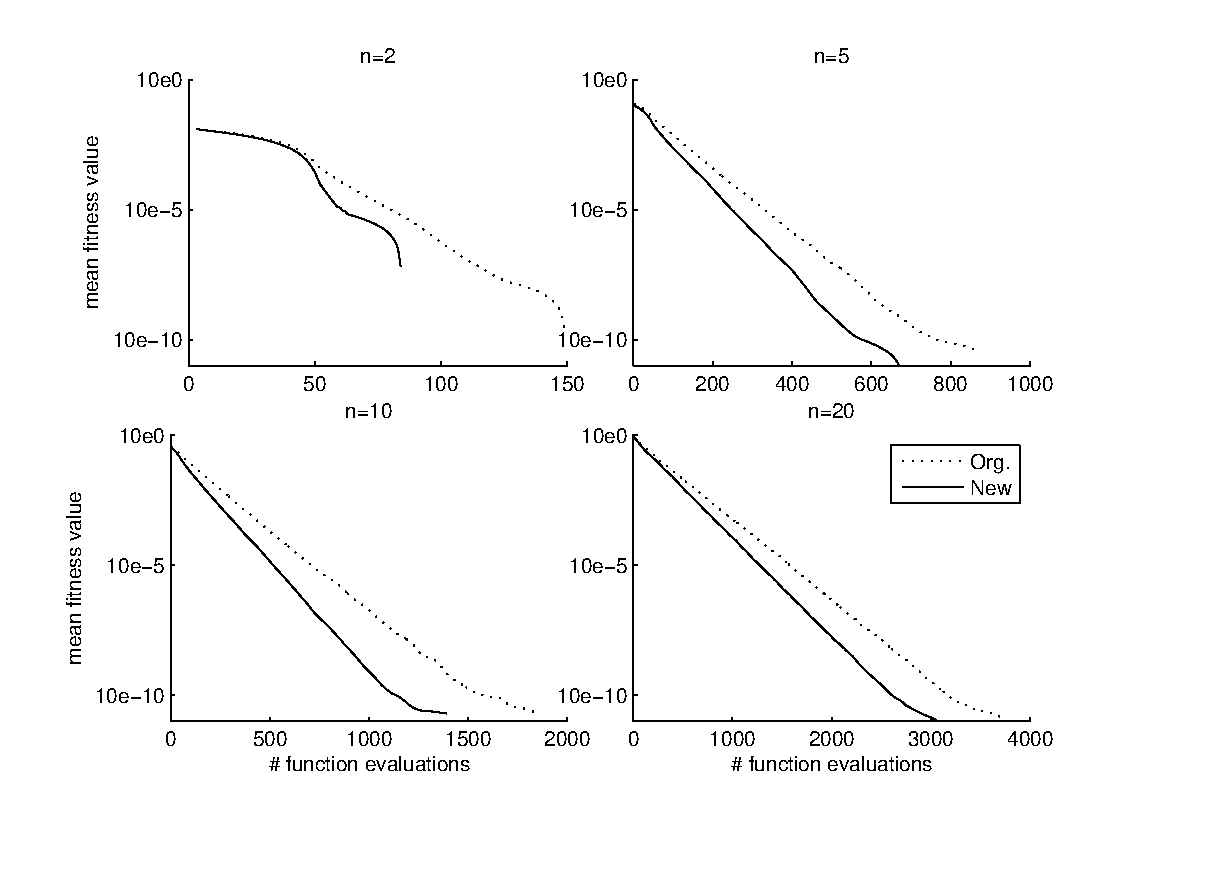
\includegraphics[trim = 10mm 10mm 10mm 5mm, clip, width=0.99\columnwidth]{figs/sphere_meanFitness_funcEval.eps}
\caption{Mean fitness values versus number of function evaluation by validating using the original method in \cite{Ru06:PPSN} (dotted) or the new and improved method from Fig.~\ref{fig:improvedmodel} (solid), for the sphere model.}
\label{fig:sphereFitness}
\end{figure}
\begin{figure}[t!]
\centering
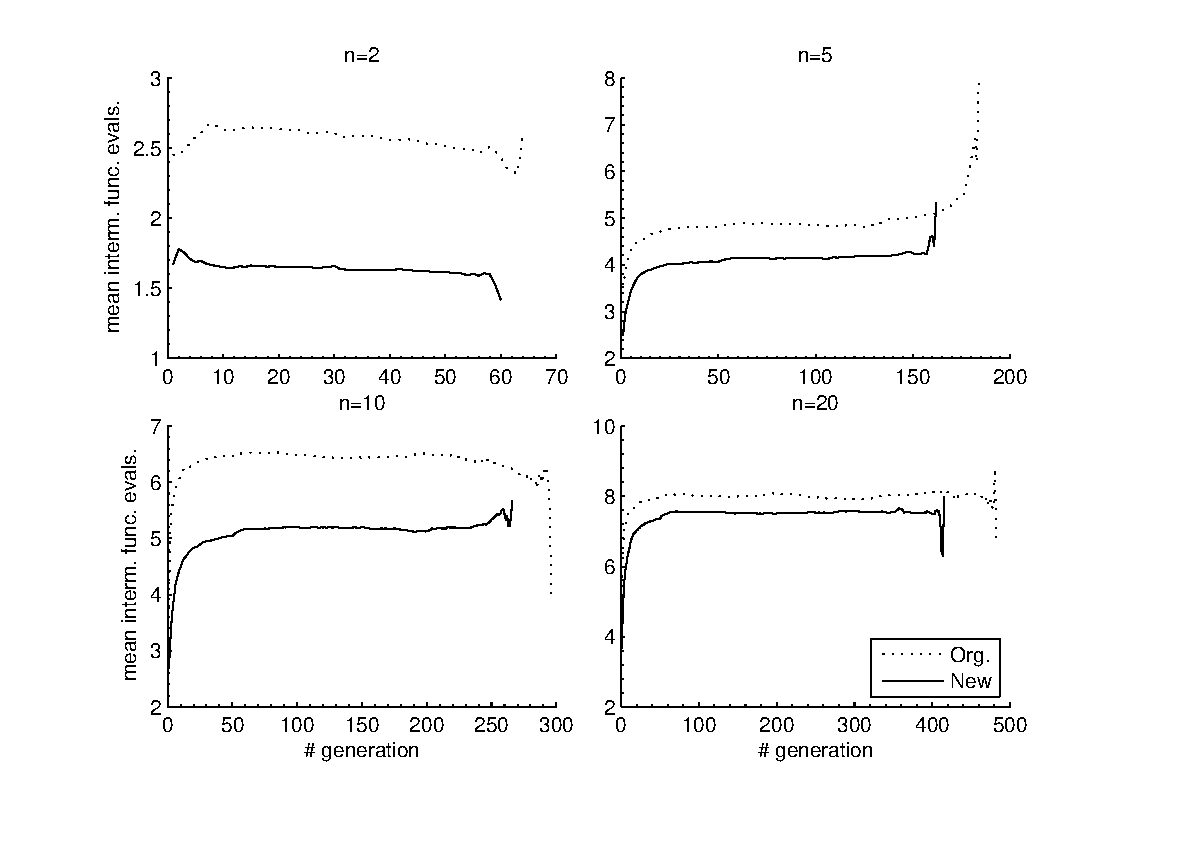
\includegraphics[trim = 10mm 10mm 10mm 5mm, clip, width=0.99\columnwidth]{figs/sphere_intmEvals_gen.eps}
\caption{Mean intermediate function evaluations versus generation by validating using the original method in \cite{Ru06:PPSN} (dotted) or the new and improved method from Fig.~\ref{fig:improvedmodel} (solid), for the sphere model.}
\label{fig:sphereIntmEval}
\end{figure}

\begin{table}[t!] 
\centering
{\renewcommand{\arraystretch}{1.1} \renewcommand{\tabcolsep}{0.05cm} \scriptsize%footnotesize
\begin{tabularx}{0.99\columnwidth}{| X | c | rrr | rrr| rrr |}
\hline
 & & \multicolumn{3}{c|}{Function eval.} & \multicolumn{3}{c|}{Generations} & \multicolumn{3}{c|}{Fitness} \\ 
     & $n$ & \multicolumn{1}{|c}{mean} & \multicolumn{1}{c}{median} & \multicolumn{1}{c|}{std} & \multicolumn{1}{|c}{mean} & \multicolumn{1}{c}{median} & \multicolumn{1}{c|}{std} & \multicolumn{1}{|c}{mean} & \multicolumn{1}{c}{median} & \multicolumn{1}{c|}{std} \\
\hline
org& 2 & 130.59 & 132 & 18.33 & 49.02 & 49 & 6.51 & 2.35e-09 & 2.82e-10 & 1.15e-08\\ 
new&2 & 81.53 & 81 & 9.53 & 48.11 & 48 & 5.02 & 7.01e-10 & 2.26e-10 & 1.35e-09\\ \hline
org& 5 & 702.02 & 702 & 67.57 & 145.15 & 145 & 14.96 & 2.77e-10 & 1.82e-10 & 3.64e-10\\ 
new& 5 & 545.25 & 547 & 54.27 & 132.60 & 132 & 11.03 & 1.83e-10 & 1.46e-10 & 1.09e-10\\ \hline
org& 10 & 1563.58 & 1553 & 117.09 & 241.83 & 240 & 18.47 & 1.52e-10 & 1.37e-10 & 5.03e-11\\ 
new& 10 & 1161.03 & 1158 & 79.98 & 226.60 & 224 & 13.86 & 1.34e-10 & 1.22e-10 & 3.80e-11\\ \hline
org& 20 & 3383.83 & 3377 & 135.52 & 423.14 & 424 & 20.42 & 1.27e-10 & 1.21e-10 & 2.51e-11\\ 
new& 20 & 2795.28 & 2804 & 132.77 & 372.86 & 372 & 16.56 & 1.17e-10 & 1.12e-10 & 1.72e-11\\ \hline
\end{tabularx}
}
\caption{Experimental results for mean, median and standard deviations for function evaluations, generations, 
and their corresponding fitness by validating using the original method in \cite{Ru06:PPSN} or the new and improved method from Fig.~\ref{fig:improvedmodel}, for various dimensions $n$ of the sphere model.}\label{tbl:Sphere}
\end{table}

\subsection{Rosenbrock's function}\label{sec:rosen}
The first experiment is now repeated for the Rosenbrock's function, 
\begin{equation}f(\vec{x}) = \sum_{i=2}^n 100(x_{i}-x_{i-1}^2)^2 + (1-x_{i-1})^2.\end{equation}
The average fitness versus the number of function evaluations is presented in Fig.~\ref{fig:rosenFitness} and Fig.~\ref{fig:rosenIntmEval} shows the mean intermediate function evaluations that are calculated during the validation process. Despite requiring more generations, the over all function evaluations are significantly lower and yield a better fitness when using the method presented in Fig.~\ref{fig:improvedmodel} as shown in Table~\ref{tbl:Rosenbrock}. If all of the candidate points have to be ranked correctly, the method will get stuck in local minima for this problem in around 6 out of 100 experiments, however this is not a problem if only the $\mu$ best candidate points are ranked consistently, except at high dimensions, and even then the $\mu$ best points policy significantly outperforms evaluating all of the candidate points. Clearly the choice of validation policy will influence search performance. 
\begin{figure}[b!]
\centering
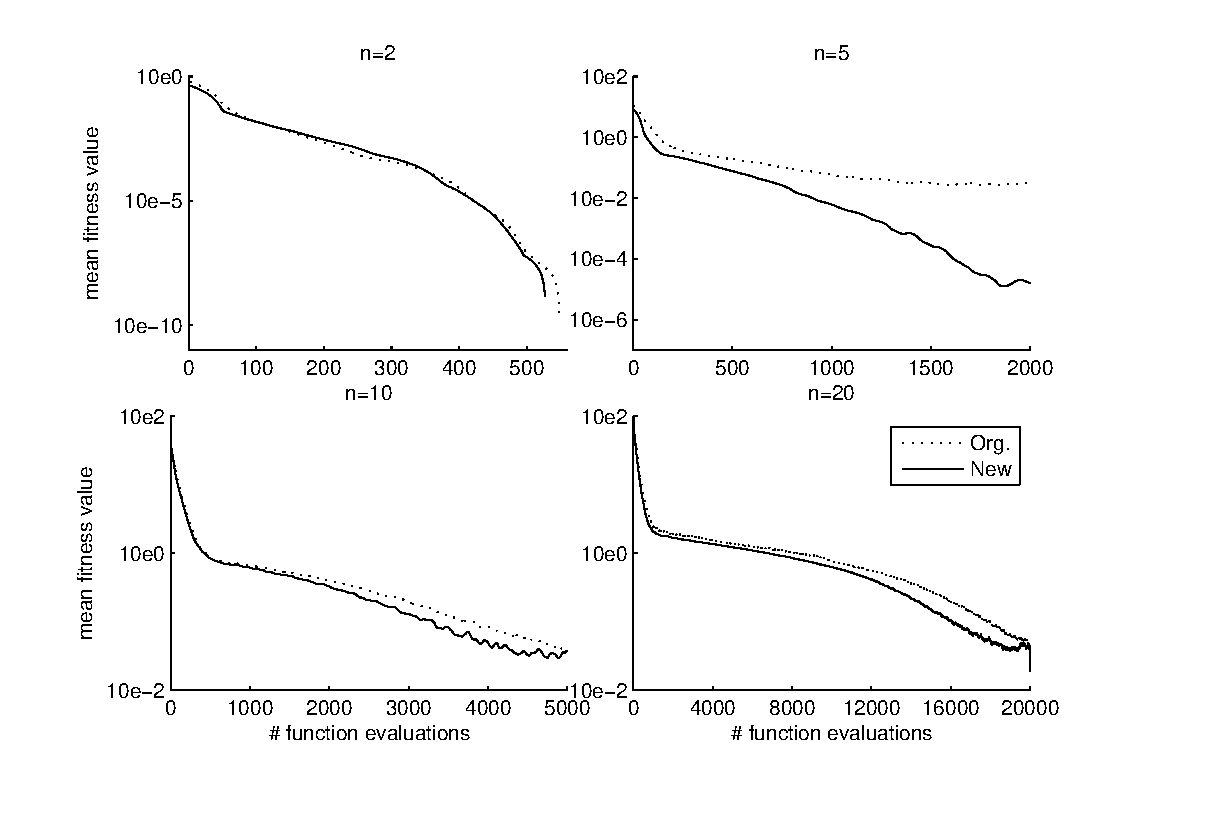
\includegraphics[trim = 10mm 10mm 10mm 5mm, clip, width=0.99\columnwidth]{figs/rosen_meanFitness_funcEval.eps}
\caption{Mean fitness values versus number of function evaluation by validating using the original method in \cite{Ru06:PPSN} (dotted) or the new and improved method from Fig.~\ref{fig:improvedmodel} (solid), for the Rosenbrock's function.}
\label{fig:rosenFitness}
\end{figure}
\begin{figure}[t!]
\centering
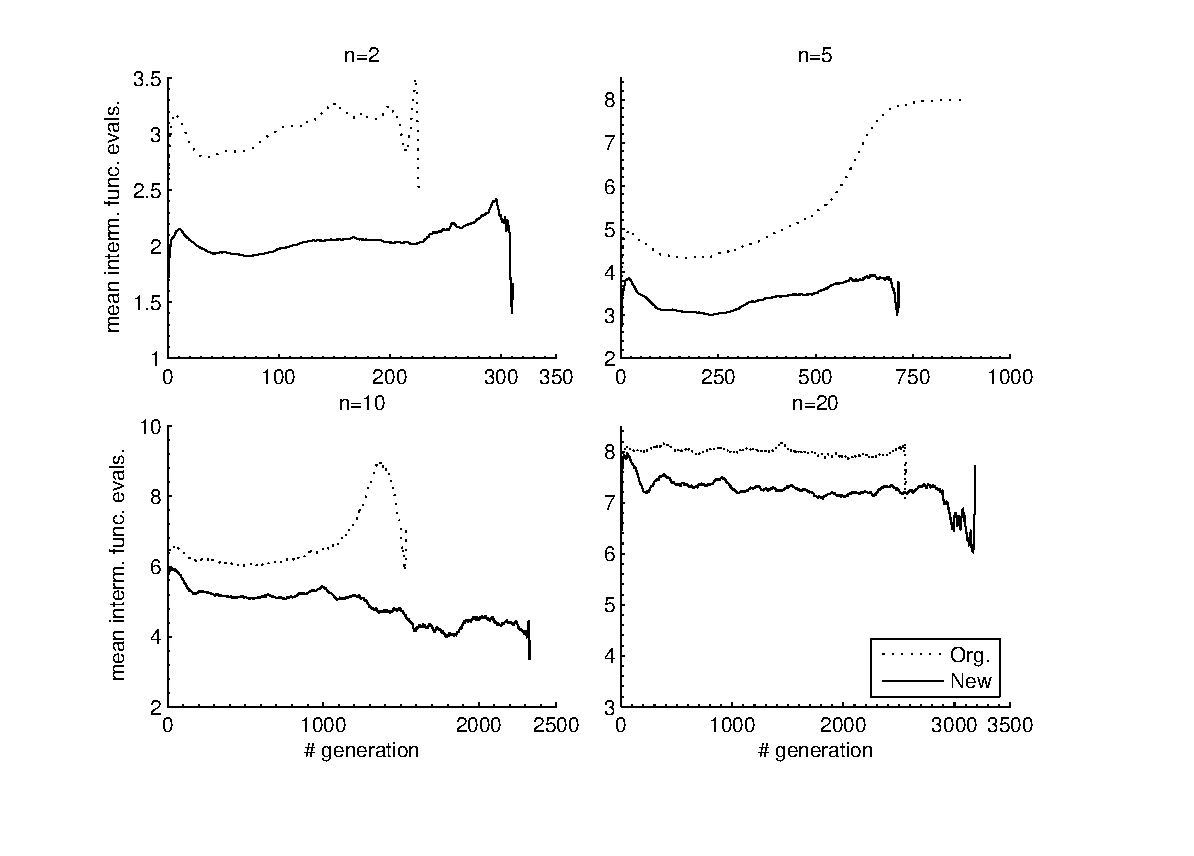
\includegraphics[trim = 15mm 10mm 15mm 5mm, clip, width=0.99\columnwidth]{figs/rosen_intmEvals_gen.eps}
\caption{Mean intermediate function evaluations versus generation by validating using the original method in \cite{Ru06:PPSN} (dotted) or the new and improved method from Fig.~\ref{fig:improvedmodel} (solid), for the Rosenbrock's function.}
\label{fig:rosenIntmEval}
\end{figure}

\begin{table}[t!]
\centering
{\renewcommand{\arraystretch}{1.1} \renewcommand{\tabcolsep}{0.03cm} \scriptsize%footnotesize
\begin{tabularx}{0.99\columnwidth}{| X | c | rrr | rrr| rrr |}
\hline
 & & \multicolumn{3}{c|}{Function eval.} & \multicolumn{3}{c|}{Generations} & \multicolumn{3}{c|}{Fitness} \\ 
     & $n$ & \multicolumn{1}{|c}{mean} & \multicolumn{1}{c}{median} & \multicolumn{1}{c|}{std} & \multicolumn{1}{|c}{mean} & \multicolumn{1}{c}{median} & \multicolumn{1}{c|}{std} & \multicolumn{1}{|c}{mean} & \multicolumn{1}{c}{median} & \multicolumn{1}{c|}{std} \\
\hline
org & 2 & 389.85 & 386 & 63.85 & 132.31 & 130 & 31.25 & 6.24e-10 & 3.20e-10 & 1.05e-09\\ 
new & 2 & 344.91 & 336 & 78.58 & 172.16 & 170 & 49.95 & 7.53e-10 & 1.66e-10 & 3.64e-09\\ \hline
org & 5 & 2464.22 & 2280 & 748.55 & 514.59 & 492 & 105.77 & 2.75e-01 & 1.74e-10 & 1.01e+00\\ 
new & 5 & 1724.89 & 1729 & 295.60 & 520.66 & 520 & 82.79 & 1.83e-10 & 1.53e-10 & 1.05e-10\\ \hline
org & 10 & 6800.50 & 6495 & 1258.68 & 1079.82 & 1052 & 177.76 & 2.79e-01 & 1.32e-10 & 1.02e+00\\ 
new & 10 & 6138.48 & 6143 & 1398.15 & 1177.71 & 1103 & 310.11 & 1.99e-01 & 1.24e-10 & 8.73e-01\\ \hline
org & 20 & 19968.80 & 20004 & 234.66 & 2494.00 & 2500 & 49.60 & 4.54e-01 & 2.88e-02 & 1.08e+00\\ 
new & 20 & 19645.90 & 20002 & 1086.37 & 2687.25 & 2748 & 230.50 & 3.10e-01 & 3.12e-07 & 9.97e-01\\ \hline
\end{tabularx}
}
\caption{Experimental results for mean, median and standard deviations for function evaluations, generations, 
and their corresponding fitness by validating using the original method in \cite{Ru06:PPSN} or the new and improved method from Fig.~\ref{fig:improvedmodel}, for various dimensions $n$ of the Rosenbrock's function.} \label{tbl:Rosenbrock}
\end{table}

\section{Discussion and Conclusion}\label{sec:Discussion}
The technique presented in this paper to control the number of true fitness evaluations is based on a single test point chosen from a set of candidate points which the surrogate ranks the highest. The approximate ranking of this test point is compared with its true ranking in order to determine the quality of the surrogate. This is a simple form of cross-validation. An alternative approach could be to rank all candidate points along with the training points using the surrogate model. This is followed by the re-ranking of training and candidate points using the updated surrogate and comparing it with the previous estimate by computing Kendall's $\tau$. Its aim is to observe a change in ranking between successive updates of the surrogate. This study has shown that during the validation process it is sufficient for $\tau$ to be close to $1$ or that only the potential parent points should be ranked consistently. Moreover, the new validation approach reduces the number of fitness evaluation needed, without a loss in performance although it might take a few more iterations in the CMA-ES algorithm. The studies presented are exploratory in nature and clearly the approach must be evaluated on a greater range of evolutionary tasks. These investigations are currently underway. 

When it comes to modeling surrogates based on training data, the general rule of thumb is bigger the training set, the more accurate a model. However, there are computational time limits thus pruning of the training set is necessary. Previous studies \cite{Jin2005,Ratle1999} have reported that replacing random training points is not optimal. This study has shown that there is no statistical difference in omitting oldest or lowest-ranking points from the training set. Hence, for future work, further investigation on the fitness landscape is needed to determine effectively which search area is no longer of interest and thus unnecessary for the surrogate to approximate correctly. For instance it could be of interest to disregard training points with the largest euclidean distance away from the current candidate points rather than simply omitting the oldest/lowest-ranking training points. 

When building surrogates in evolutionary computation one is interested in the quality of ranking of points only. For this reason the training accuracy and cross validation is a more meaningful measure of quality for the surrogate model. This is in contrast to regression, where the fitness function is modeled directly and the quality estimated in terms of measures such a least square error. 
This study has shown that the sampling used for validating the accuracy of the surrogate can stop once the $\mu$ best ranked candidate points have been evaluated, since they are the only candidate points who will survive to become parents in the next generation. 
Although in some cases the sampling could stop sooner, when the surrogate ranking and true ranking were sufficiently concordant, i.e. $\tau$ was close to 1. This slight slack in for $\tau$ is allowed due to the fact the ES search is stochastic, however the allowable range in slack for $\tau$ needs to be investigated more fully. 

However, in the context of surrogate-assisted optimization the discrepancy between the exact model and its surrogate can be translated as noise, which could be an indicator of the necessary sampling size for validation/updating the surrogate, instead of only focusing on consistently ranking the $\mu$ best candidate points. Therefore one can take inspiration from a varying random walk population model suggested by \cite{Miller1997} to approximate the population sizing to overcome unnecessary fitness evaluations.



\bibliographystyle{IEEEtran}
\bibliography{biblio}

\end{document}
